\documentclass[12pt]{article}

\usepackage{amsmath}
\numberwithin{figure}{section}

\usepackage{array}
\usepackage{caption}
\usepackage[top=1in, bottom=1in, left=0.75in, right=0.75in]{geometry}

\usepackage{graphicx}
\graphicspath{{figures/}}

\usepackage[colorlinks=true, allcolors=blue]{hyperref}
\usepackage[utf8]{inputenc}
\usepackage{minted}
\usepackage{multirow}
\usepackage{nameref}
\usepackage{pdfpages}
\usepackage[section]{placeins}

\begin{document}

\begin{titlepage}
  \begin{center} \LARGE
    \vspace*{1.5in}

    ECE 272 Lab 6

    Fall 2018

    \vfill

    Video Graphics Array (VGA)

    Phi Luu

    \vfill

    November 30\textsuperscript{th}, 2018

    Grading TA: Edgar Perez

    Lab Partner: Benjamin Geyer

    \vspace{1.5in}
  \end{center}
\end{titlepage}

%%%%%%%%%%%%%%%%%%%%%%%%%%%%%%%%%%%%%%%%%%%%%%%%%%%%%%%%%%%%%%%%%%%%%%%%%%%%%%%%
% Introduction
%%%%%%%%%%%%%%%%%%%%%%%%%%%%%%%%%%%%%%%%%%%%%%%%%%%%%%%%%%%%%%%%%%%%%%%%%%%%%%%%
\section{Introduction}

\textit{Video graphics array} (\textit{VGA}) is a graphics standard for video display controller first introduced by IBM in 1987. VGA can be used to display a wide range of resolutions and refresh rates. VGA draws on the monitor from left to right and top to bottom. Each pixel is controlled by three analog pins for red, green, and blue (RGB) channels. Although VGA can control a wide range of resolutions and refresh rates, the 640x480 60Hz configuration is commonly used.

For the DE10-Lite, each of the RGB channels is a 4-bit port. The red, green, and blue channels connect to pins 1, 2, and 3 of the VGA connector, respectively. The horizontal sync (hsync) and vertical sync (vsync) signals of the FPGA connect to pins 13 and 14 of the VGA connector, respectively. Hsync and vsync are active-low. When hsync goes to 0, the next line starts to draw; when vsync goes to 0, the drawer goes back to the top of the screen again, starting a new frame. Figure~\ref{fig:de10_lite_vga_pinout}.

\begin{figure}[ht]
  \centering
  \includegraphics[width=0.75\textwidth]{de10_lite_vga_pinout.png}
  \caption{Connections between the VGA and the MAX 10 FPGA}
  \label{fig:de10_lite_vga_pinout}
\end{figure}

A more detailed pinout of a VGA connector is illustrated by Figure~\ref{fig:vga_connector_pinout}.

\begin{figure}[ht]
  \centering
  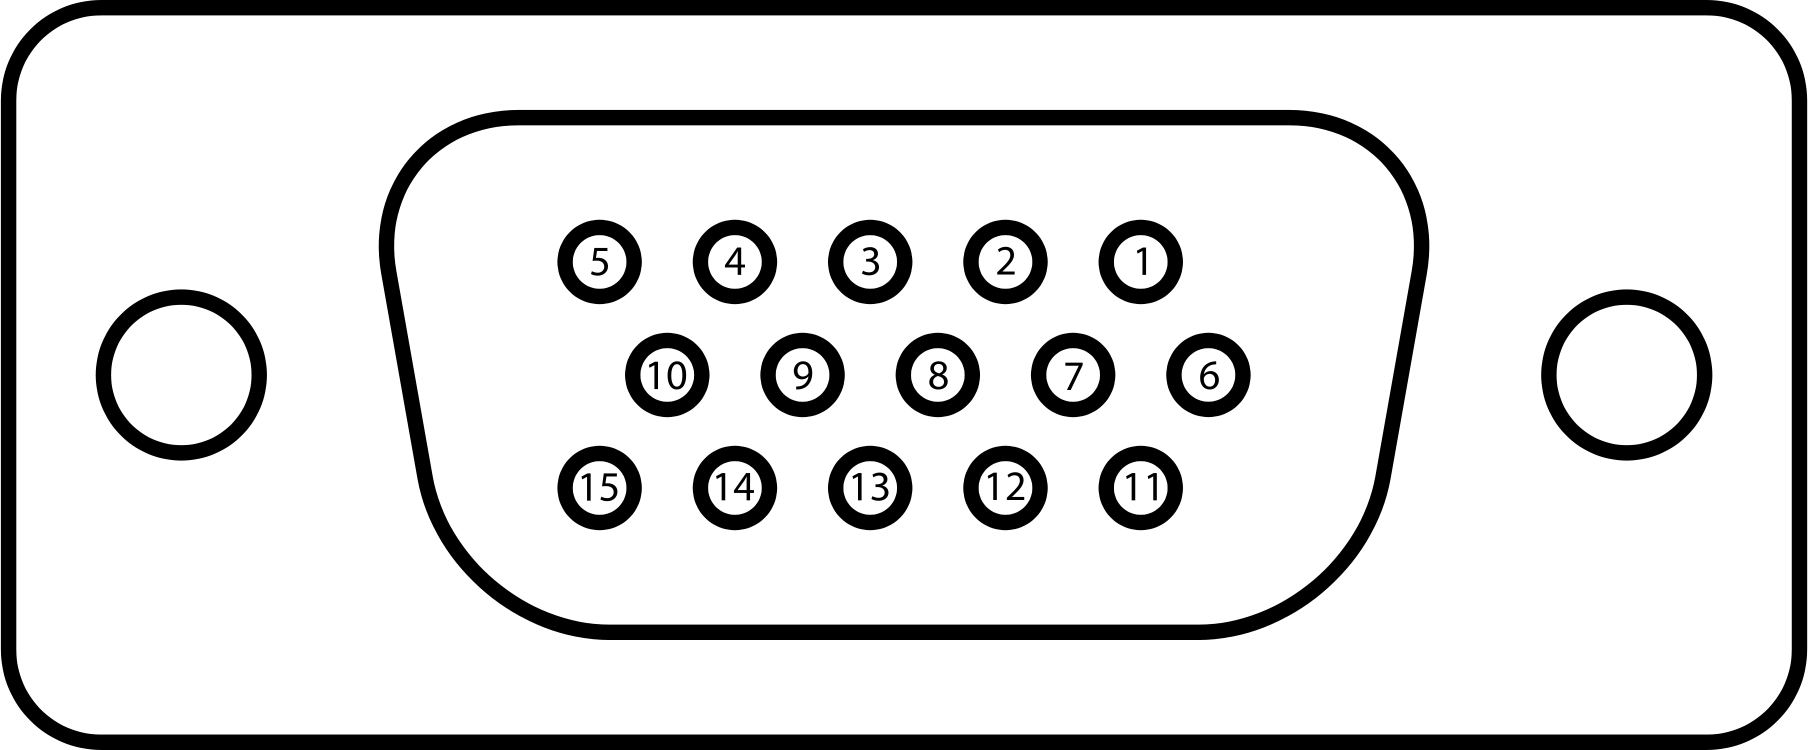
\includegraphics[width=0.45\textwidth]{vga_female_socket.png}
  \caption{All 15 pins of a VGA connector. See Table~\ref{tab:vga_pinout_table}.}
  \label{fig:vga_connector_pinout}
\end{figure}

\begin{table}[ht]
  \centering
  \begin{tabular}{ | c | c | l | }
  \hline
  \textbf{Pin} & \textbf{Signal} & \textbf{Description}                                                                     \\ \hline
  1            & RED             & Red video                                                                                \\ \hline
  2            & GREEN           & Green video                                                                              \\ \hline
  3            & BLUE            & Blue video                                                                               \\ \hline
  4            & ID2/RES         & \begin{tabular}[c]{@{}l@{}}formerly Monitor ID bit 2\\ Reserved since E-DDC\end{tabular} \\ \hline
  5            & GND             & Ground (H-Sync)                                                                          \\ \hline
  6            & RED\_RTN        & Red return                                                                               \\ \hline
  7            & GREEN\_RTN      & Green return                                                                             \\ \hline
  8            & BLUE\_RTN       & Blue return                                                                              \\ \hline
  9            & KEY/PWR         & \begin{tabular}[c]{@{}l@{}}formerly key\\ now +5V DC\end{tabular}                        \\ \hline
  10           & GND             & Ground (V-Sync, DDC)                                                                     \\ \hline
  11           & ID0/RES         & \begin{tabular}[c]{@{}l@{}}formerly Monitor ID bit 0\\ reserved since E-DDC\end{tabular} \\ \hline
  12           & ID1/SDA         & \begin{tabular}[c]{@{}l@{}}formerly Monitor ID bit 1\\ PC data since DDC2\end{tabular}   \\ \hline
  13           & HSync           & Horizontal sync                                                                          \\ \hline
  14           & VSync           & Vertical sync                                                                            \\ \hline
  15           & ID3/SCL         & \begin{tabular}[c]{@{}l@{}}formerly Monitor ID bit 3\\ I2C clock since DDC2\end{tabular} \\ \hline
  \end{tabular}
  \caption{VGA pinout}
  \label{tab:vga_pinout_table}
\end{table}

%%%%%%%%%%%%%%%%%%%%%%%%%%%%%%%%%%%%%%%%%%%%%%%%%%%%%%%%%%%%%%%%%%%%%%%%%%%%%%%%
% Design
%%%%%%%%%%%%%%%%%%%%%%%%%%%%%%%%%%%%%%%%%%%%%%%%%%%%%%%%%%%%%%%%%%%%%%%%%%%%%%%%
\section{Design}

The timing sequence of an VGA controller is as follows: the pixels are displayed from left to right and top to bottom. When all the pixels of the active resolution are displayed, there is a blank period called the \textit{front porch} which signaling the start of a \textit{sync pulse}. When the front porch period finishes, the sync pulse itself is toggled from HIGH to LOW (the sync pulses are active-low). This sync pulse signals the "reset" of the xy counter: the hsync pulse resets the xy counter to the left most of the next line, whereas the vsync pulse resets the xy counter to the top left of the screen. After sync pulse period finishes, the sync pulse is toggled back to HIGH for a period of time called the \textit{back porch}.

Figure~\ref{fig:640x480_60hz_vga_timing_sequence} shows the VGA timing sequence for the 640x480 resolution with 60 Hz refresh rate.

\newpage

\begin{figure}[ht]
  \centering
  \includegraphics[width=\textwidth]{vga_timing_sequence_640x480_60hz.png}
  \caption{The display, front porch, sync pulse, and back porch signals of the horizontal timing and vertical timing of 640x480 60Hz monitor}
  \label{fig:640x480_60hz_vga_timing_sequence}
\end{figure}

Think of the timing sequence like this: the total resolution is $640 + 16 + 96 + 48 = 800$ by $480 + 33 + 2 + 10 = 525$, but the active zone is 640x480 on the top left corner of the frame.

The block diagram of the design is illustrated in Figure~\ref{fig:block_diagram} below:

\newpage

\begin{figure}[ht]
  \centering
  \includegraphics[width=\textwidth]{lab6_block_diagram.png}
  \caption{The block diagram}
  \label{fig:block_diagram}
\end{figure}

The SystemVerilog code which implements these modules is located in the \nameref{sec:appendix} section.

Putting the code through ModelSim simulation, the following results are yielded. The caption of each figure will explain the significance of the event the image captures.

\newpage

\begin{figure}[ht]
  \centering
  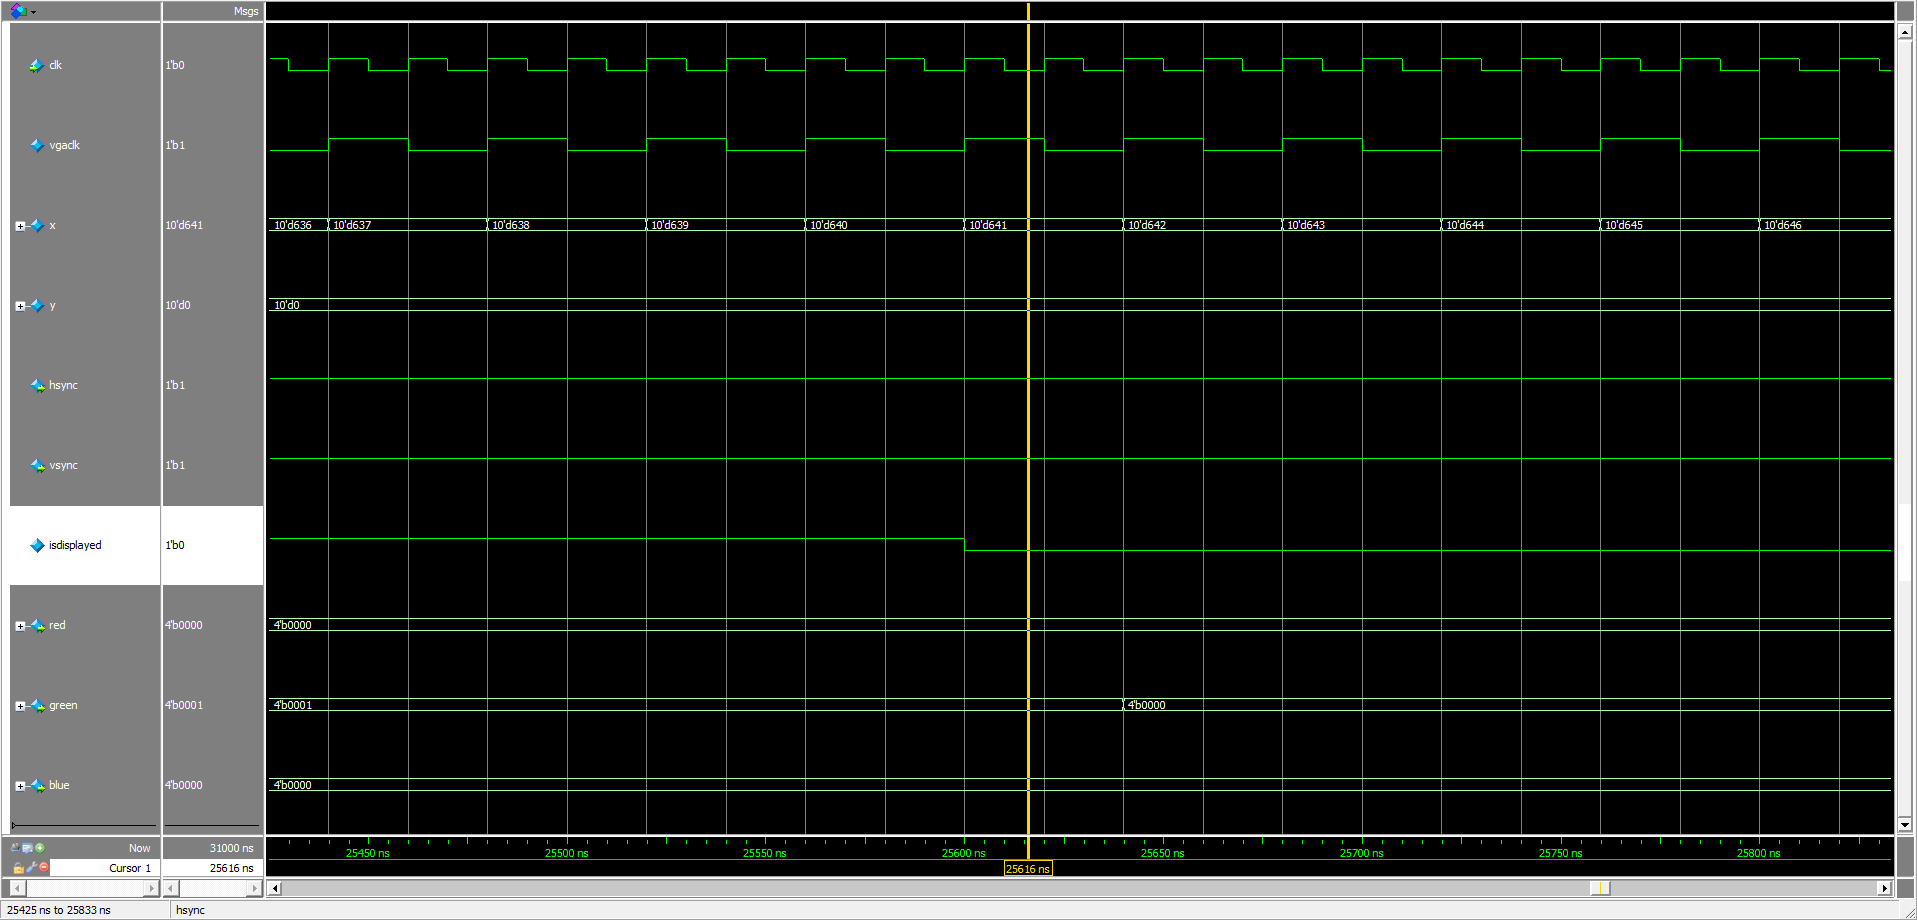
\includegraphics[width=\textwidth]{simulation_hactive_end_hfp_start.png}
  \caption{When $x$ (the horizontal counter) reaches 640, the counter goes past the active resolution, and so this is where the \textbf{horizontal front porch starts}. \href{https://i.imgur.com/QpwEYGF.jpg}{High-resolution image}}
\end{figure}

\begin{figure}[ht!]
  \centering
  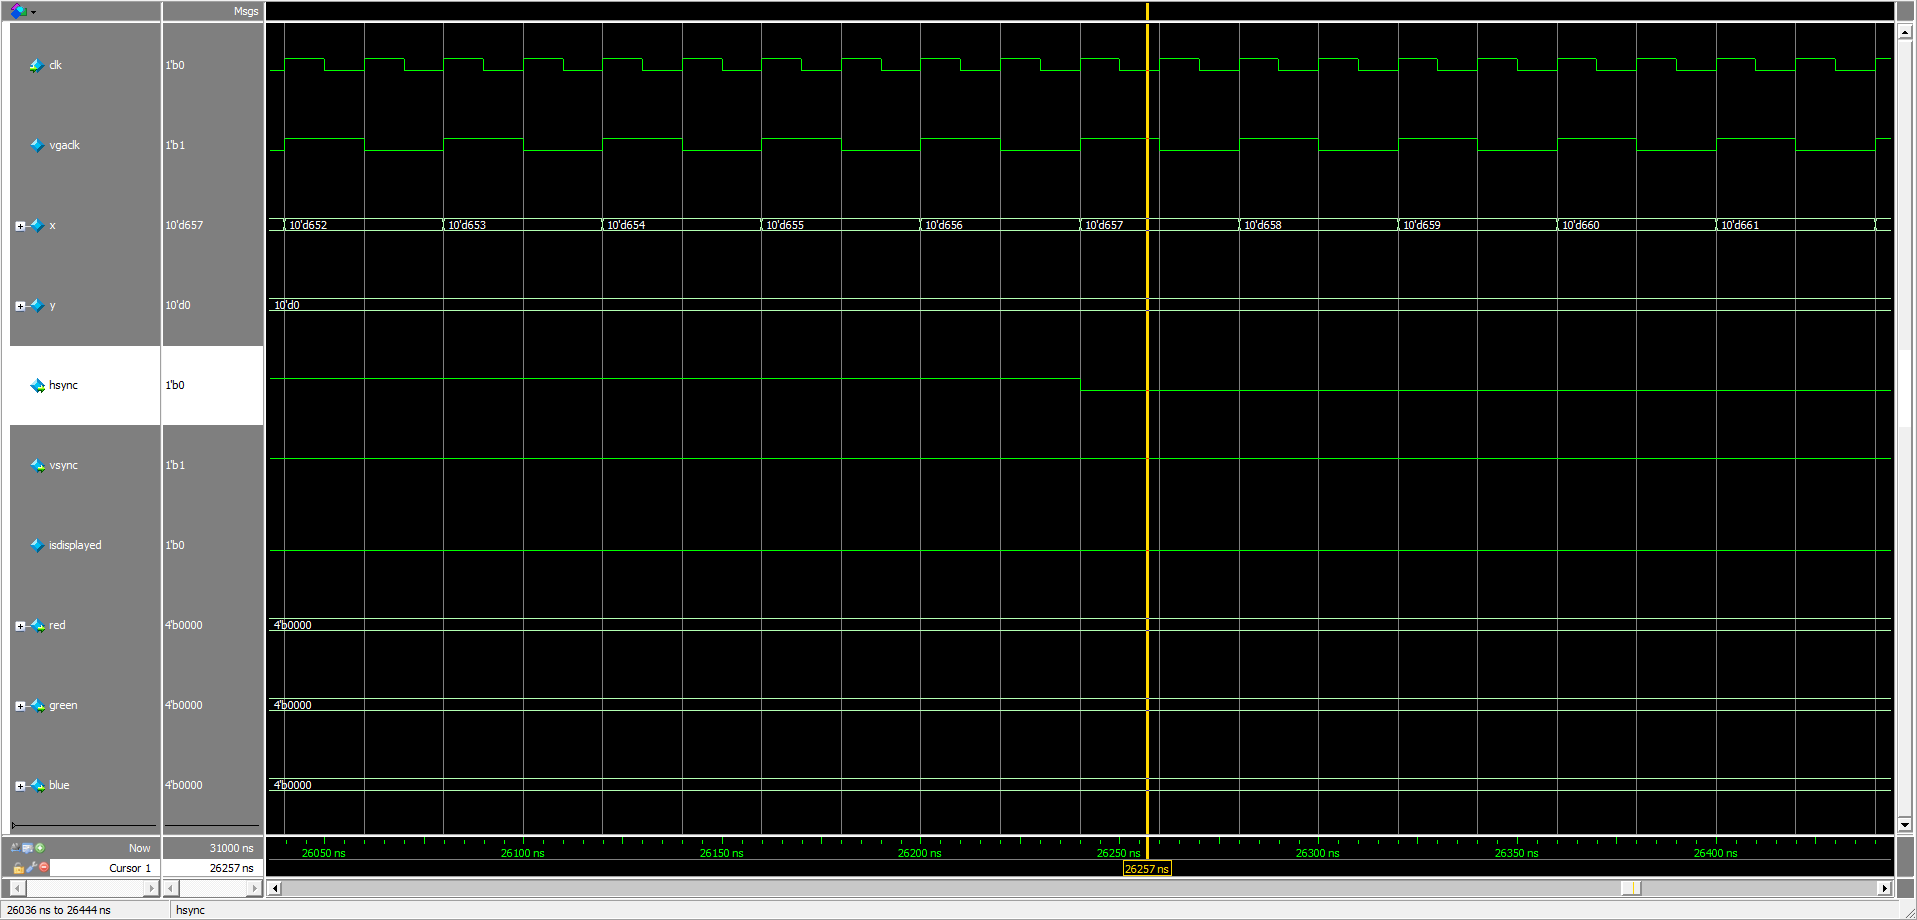
\includegraphics[width=\textwidth]{simluation_hfp_end_hsync_start.png}
  \caption{When $x$ reaches 656, the counter has gone an extra 16---which is the width of the horizontal front porch, and so this is where the \textbf{horizontal sync pulse starts going LOW}. \href{https://i.imgur.com/EfWxYUW.jpg}{High-resolution image}}
\end{figure}

\newpage

\begin{figure}[ht]
  \centering
  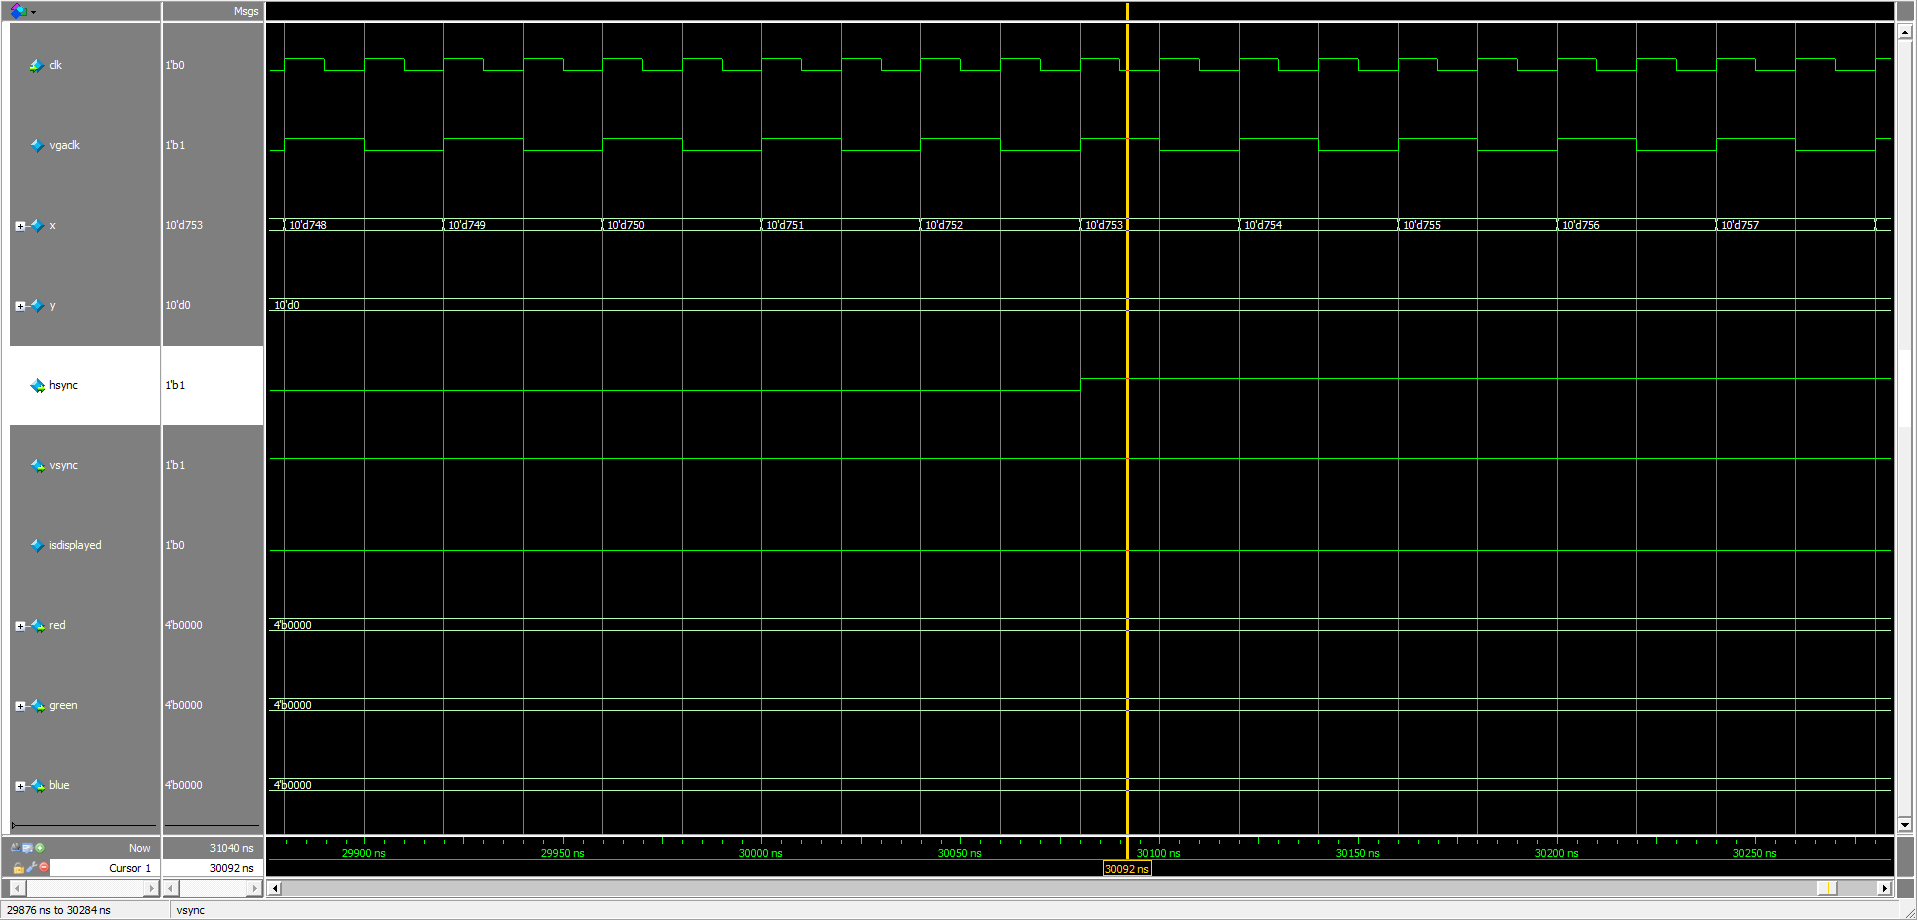
\includegraphics[width=\textwidth]{simulation_hsync_end_hbp_start.png}
  \caption{When $x$ reaches 752, the counter has gone an extra 96---which is the width of the horizontal sync pulse, and so this is where the \textbf{horizontal back porch starts}. \href{https://i.imgur.com/IkwIol1.jpg}{High-resolution image}}
\end{figure}

\begin{figure}[ht!]
  \centering
  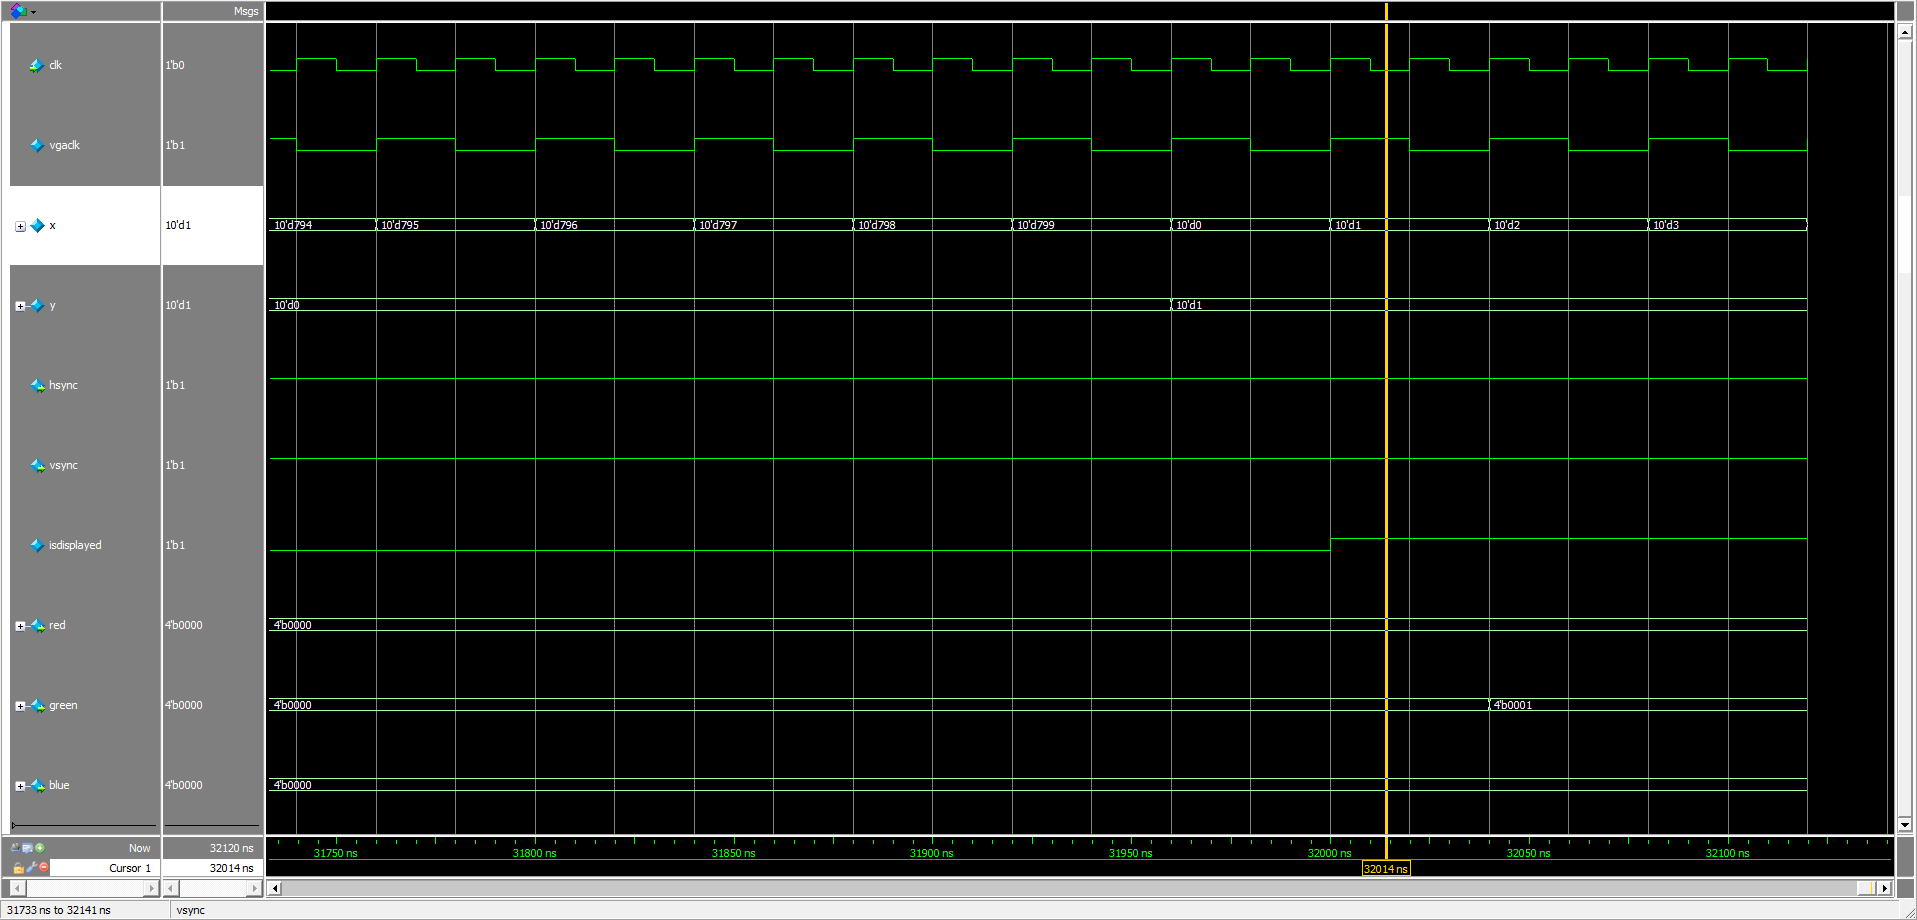
\includegraphics[width=\textwidth]{simulation_x_complete_one_line.png}
  \caption{When $x$ reaches 800, it will reset back to 0, and $y$ (the vertical counter) will increased by 1. The counters will keep counting horizontally and then vertically until the vertical counter reaches its limit. \href{https://i.imgur.com/Tqamgkr.jpg}{High-resolution image}}
\end{figure}

Similarly, the figures below show and explain how the vertical front porch, sync pulse, and back porch work.

\newpage

\begin{figure}[ht]
  \centering
  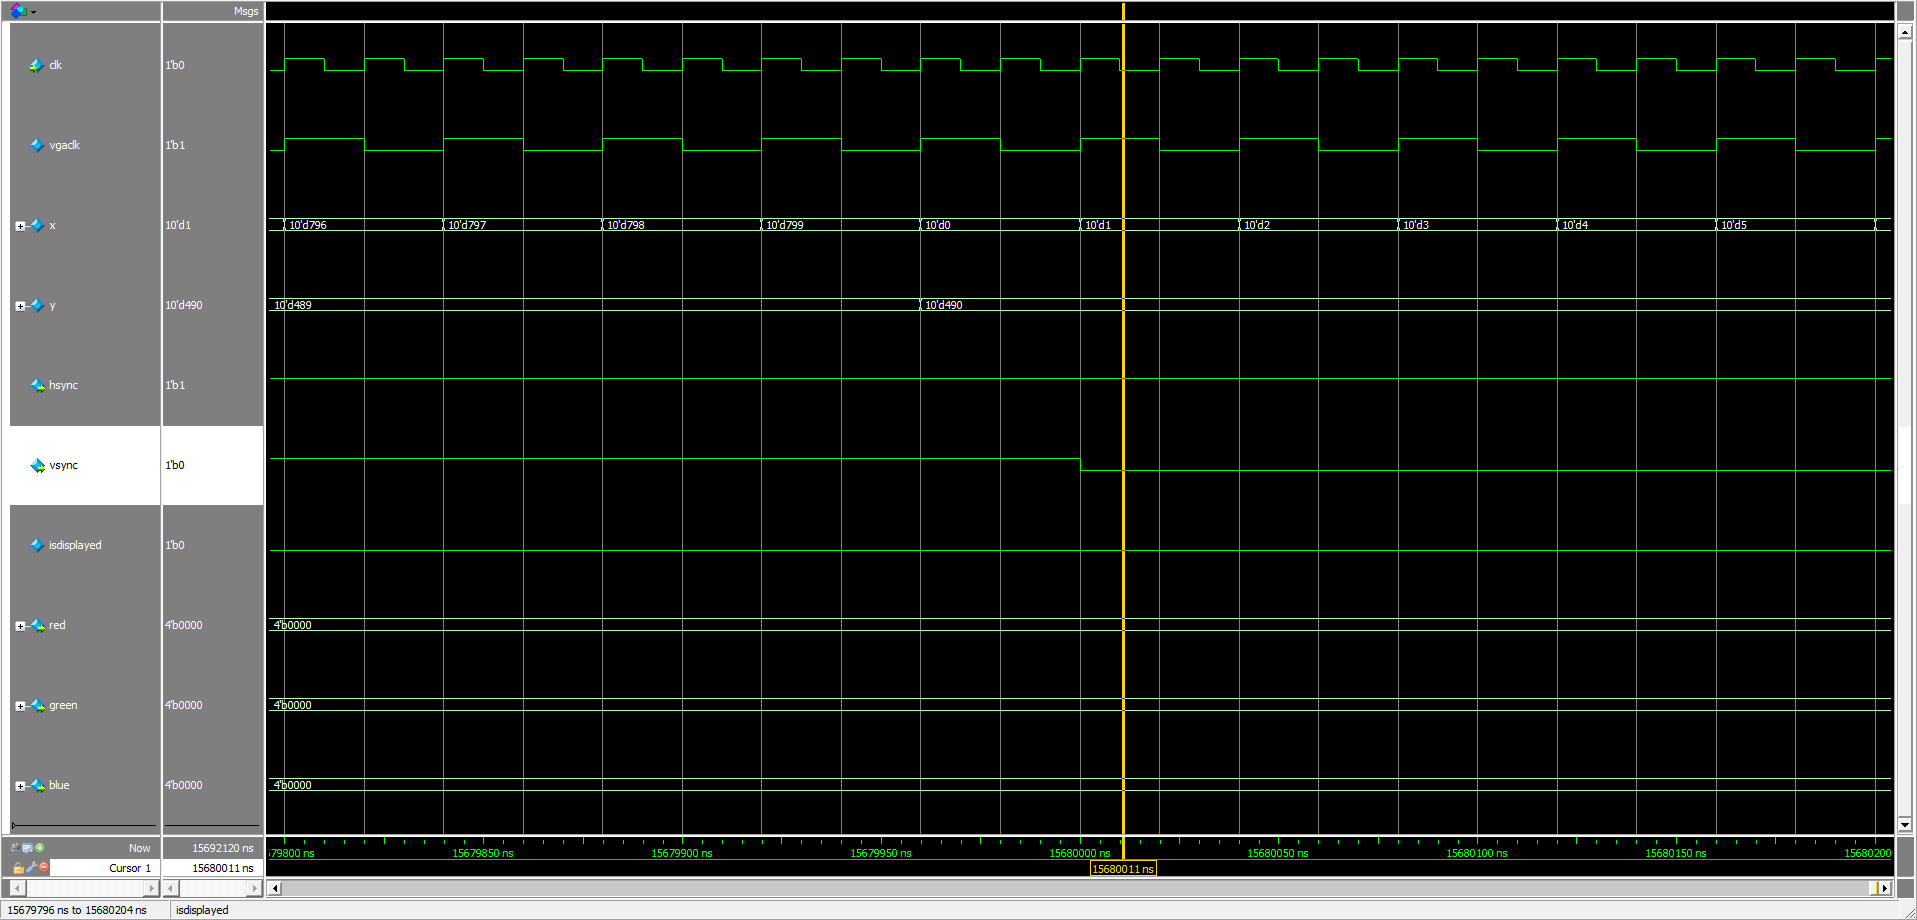
\includegraphics[width=\textwidth]{simulation_vfp_end_vsync_start.png}
  \caption{When $x$ reaches 640 and $y$ reaches 480, the counter has finished one whole active zone of the screen, and so this is where the \textbf{vertical front porch starts}. \href{https://i.imgur.com/aNPD7pG.jpg}{High-resolution image}}
\end{figure}

\begin{figure}[ht!]
  \centering
  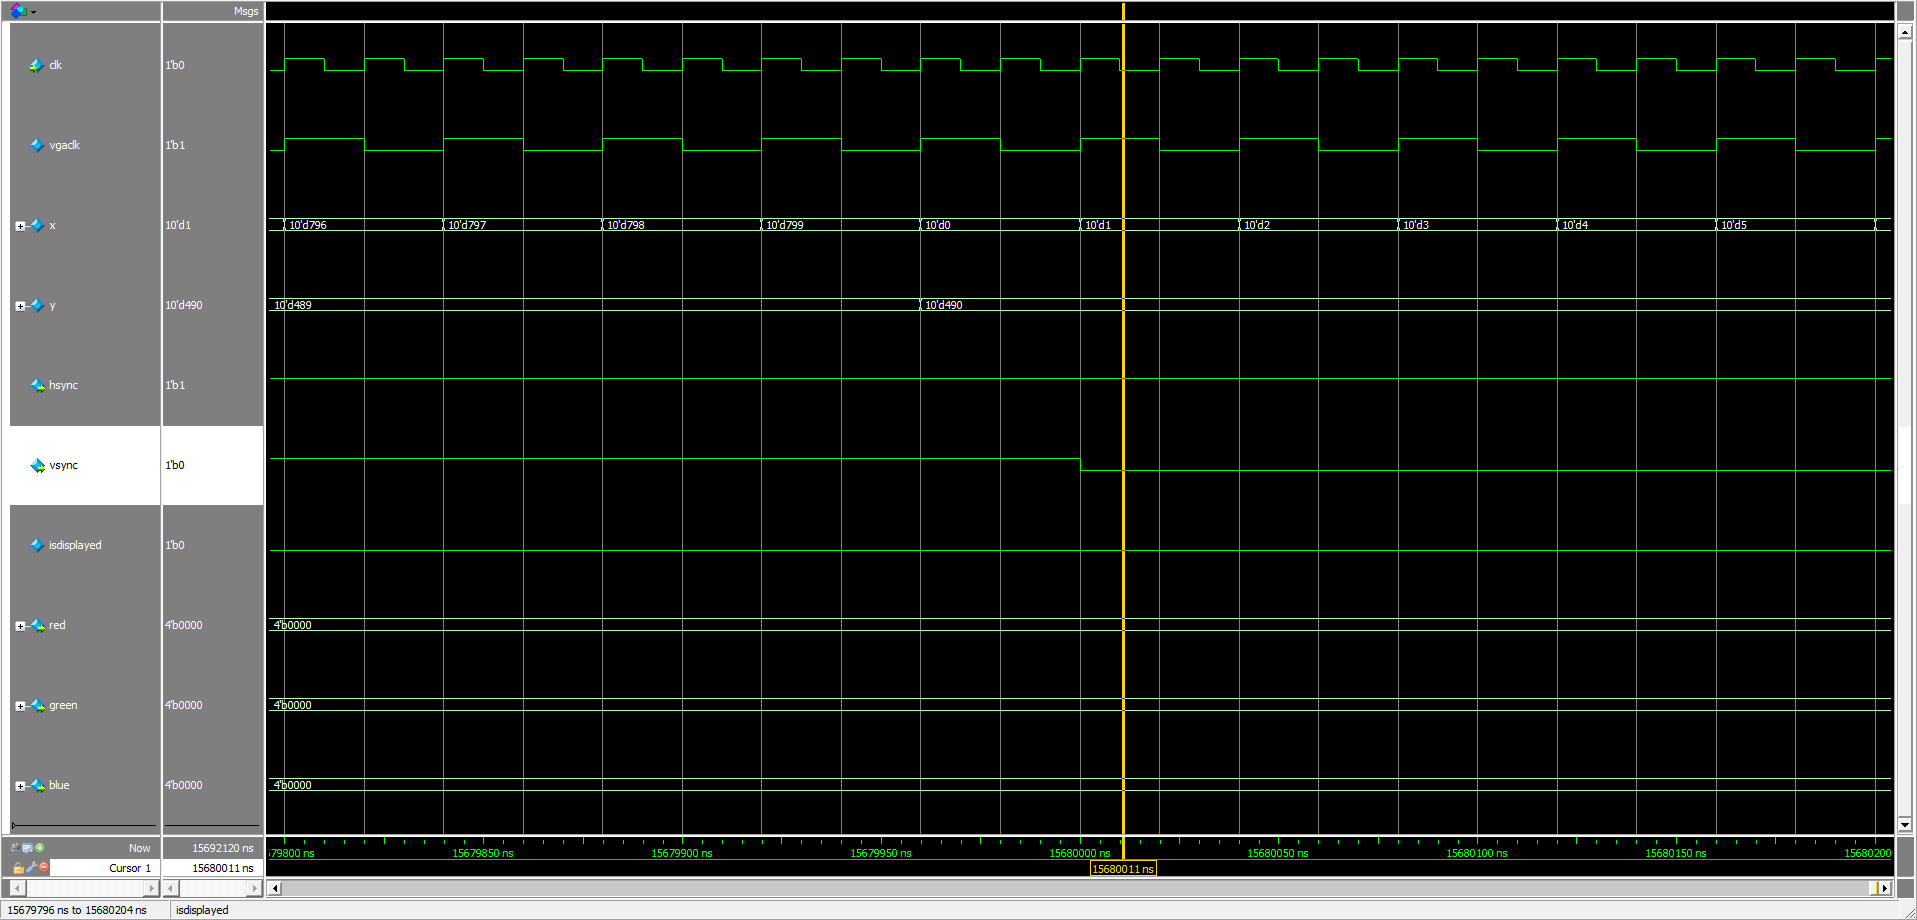
\includegraphics[width=\textwidth]{simulation_vfp_end_vsync_start.png}
  \caption{When $y$ reaches 490, the counter has gone an additional 10---which is the width of the vertical front porch, and so this is where the \textbf{vertical sync pulse starts going LOW}. \href{https://i.imgur.com/inYrF2u.jpg}{High-resolution image}}
\end{figure}

\newpage

\begin{figure}[ht]
  \centering
  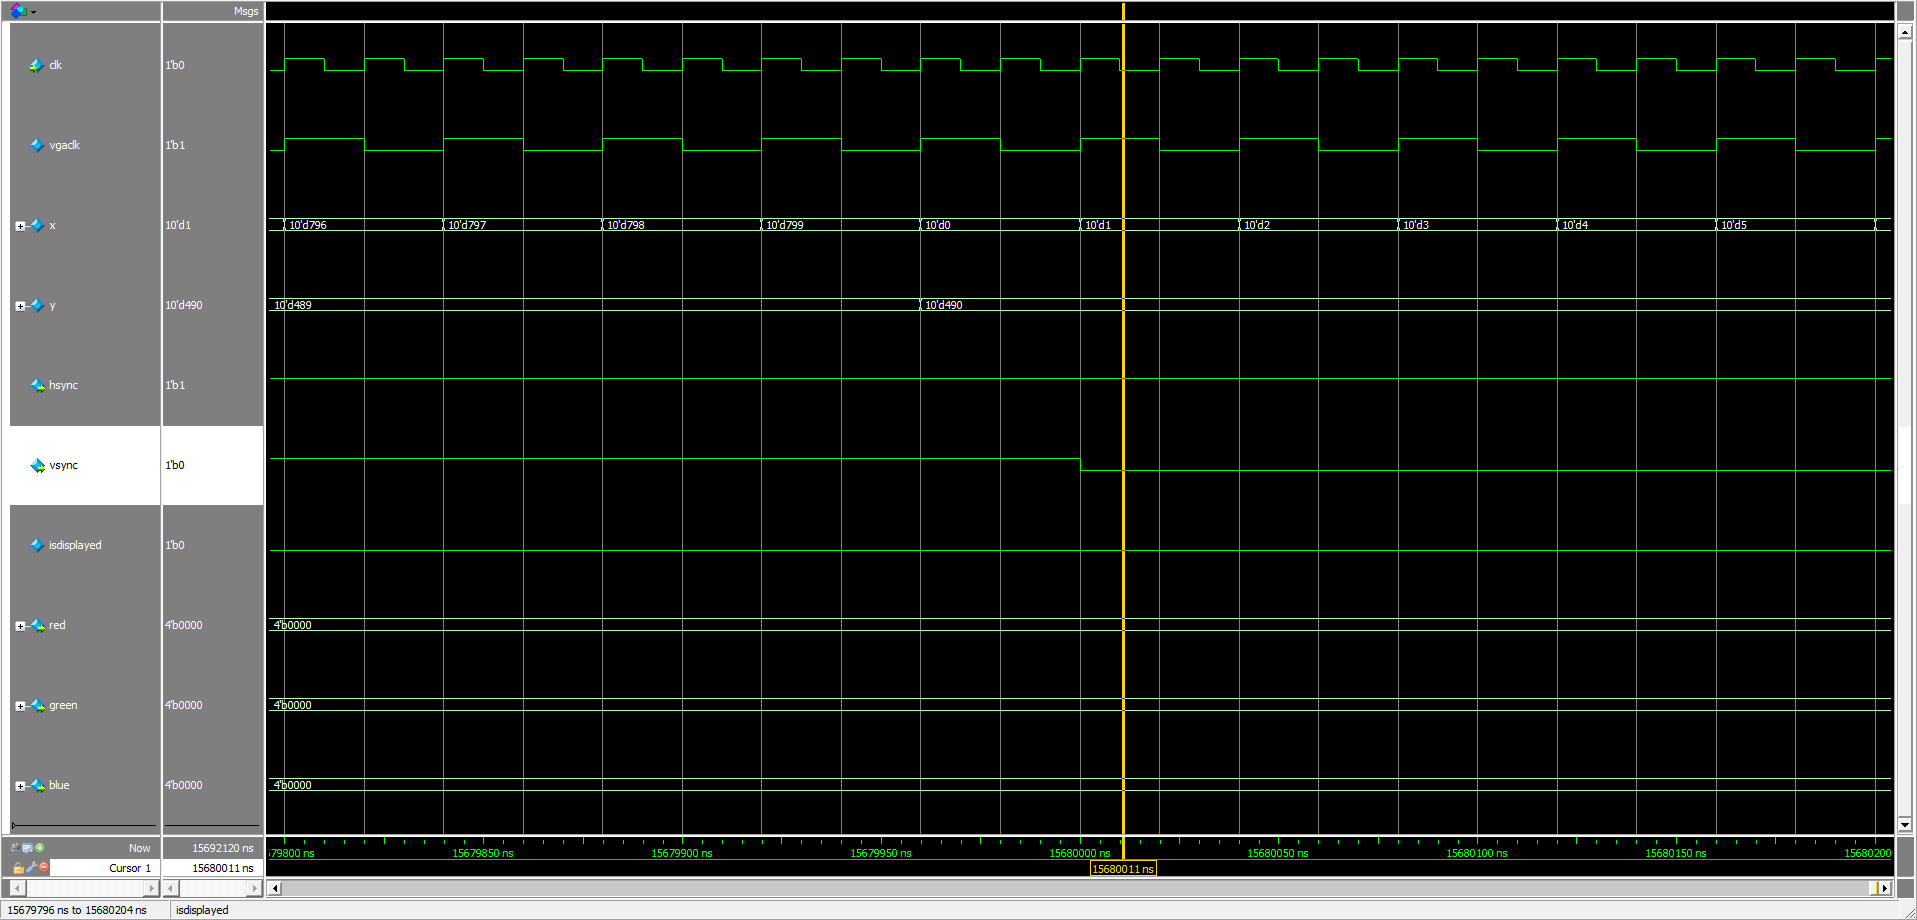
\includegraphics[width=\textwidth]{simulation_vfp_end_vsync_start.png}
  \caption{When $y$ reaches 492, the counter has gone an additional 2---which is the width of the vertical sync pulse, and so this is where the \textbf{vertical back porch starts}. \href{https://i.imgur.com/c5Ki9mq.jpg}{High-resolution image}}
\end{figure}

\begin{figure}[ht!]
  \centering
  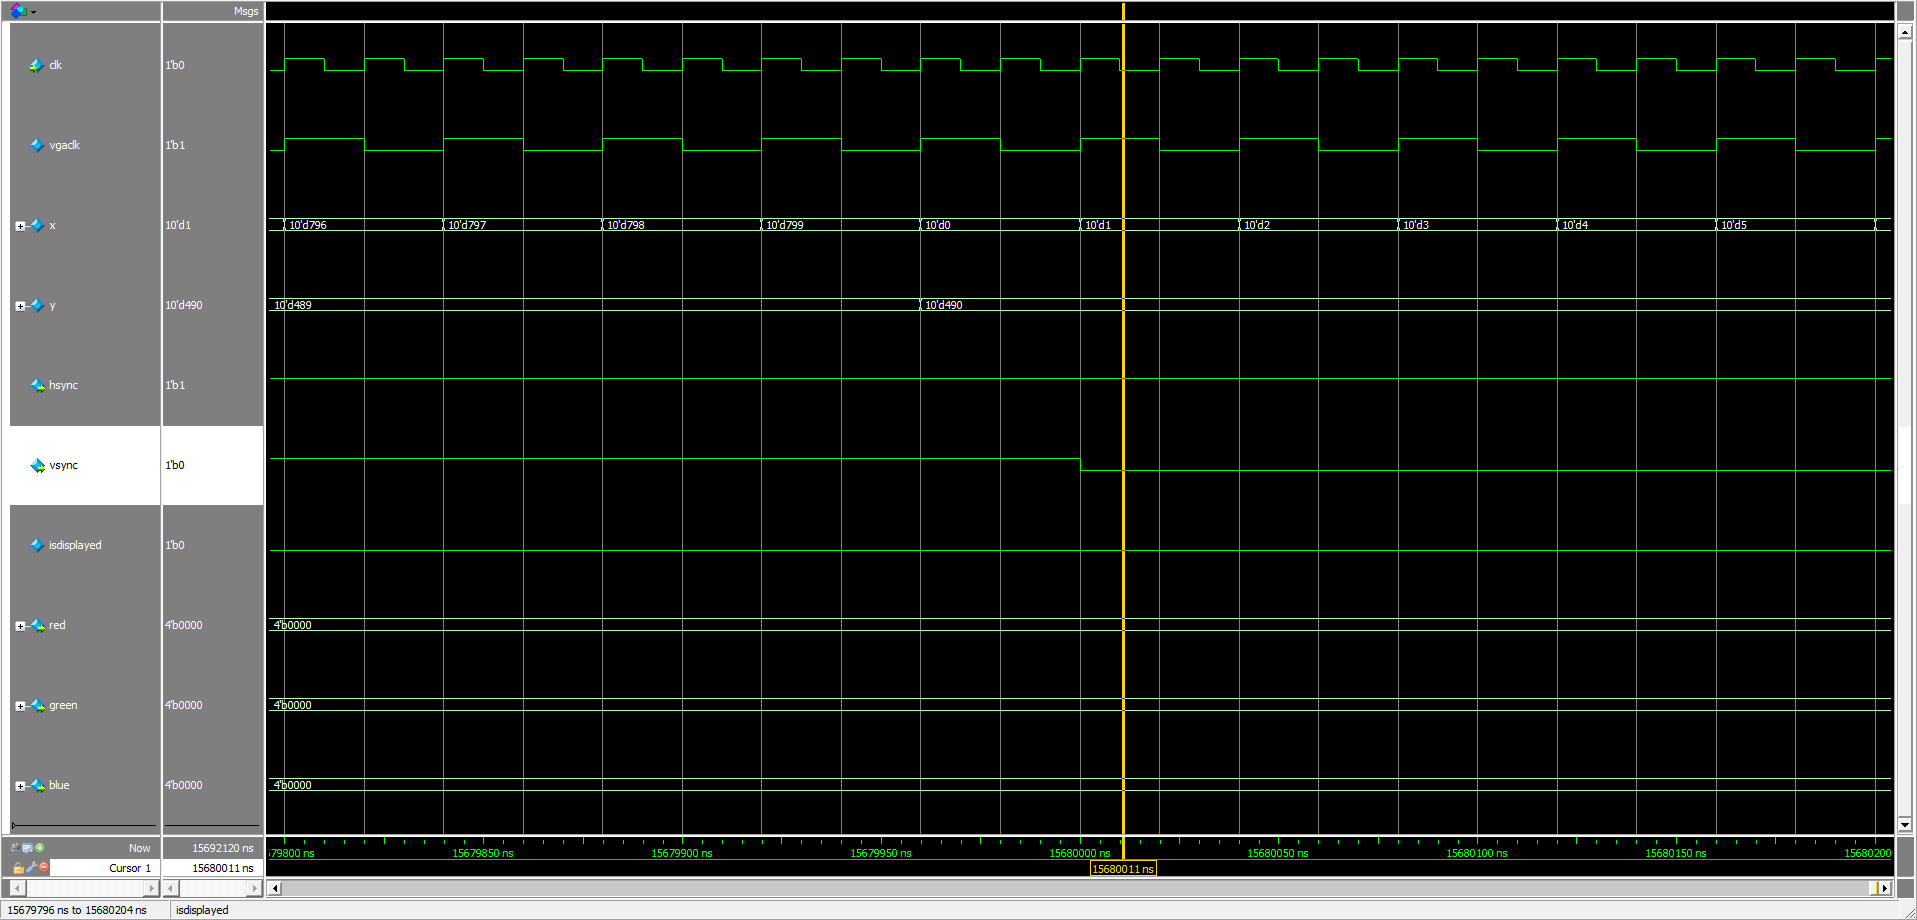
\includegraphics[width=\textwidth]{simulation_vfp_end_vsync_start.png}
  \caption{When $x$ reaches 800 and $y$ reaches 525, the counter has finished the entire screen. Since they have reached their limit, the counter will be wrapped around, and $x$ and $y$ will both reset to 0. \href{https://i.imgur.com/vl7NCR8.jpg}{High-resolution image}}
\end{figure}

\newpage

According to the figures above, the simulation yields the expected results. I uploaded the program to the FPGA and get the desired screen. Therefore, the VGA controller and drawer have been successfully implemented.

%%%%%%%%%%%%%%%%%%%%%%%%%%%%%%%%%%%%%%%%%%%%%%%%%%%%%%%%%%%%%%%%%%%%%%%%%%%%%%%%
% Experiment Notes
%%%%%%%%%%%%%%%%%%%%%%%%%%%%%%%%%%%%%%%%%%%%%%%%%%%%%%%%%%%%%%%%%%%%%%%%%%%%%%%%
\section{Experiment Notes}

%%%%%%%%%%%%%%%%%%%%%%%%%%%%%%%%%%%%%%%%
% Reflection
%%%%%%%%%%%%%%%%%%%%%%%%%%%%%%%%%%%%%%%%
\subsection*{Reflection}

This lab, particularly the timing sequence of the VGA protocol, was quite challenging. It took me more than 3 hours to finally get the timing right in SystemVerilog. The rest of the program was very easy, though. I was able to draw a red box on top of the blue background on the screen using this program.

%%%%%%%%%%%%%%%%%%%%%%%%%%%%%%%%%%%%%%%%
% Study Questions
%%%%%%%%%%%%%%%%%%%%%%%%%%%%%%%%%%%%%%%%
\subsection*{Study Questions}

\begin{enumerate}
  \item What was the toughest aspect of ECE 272? What should be changed or added to the ECE 272 manual to make this course better?

  The toughest aspect of ECE 272 was the SystemVerilog tasks. It was difficult to do sequential logic and timing in SystemVerilog, especially the SPI and the VGA labs. A suggestion to make ECE 272 better is to add starter code into the lab manual, at least for the SPI and the VGA labs.

  \item What would you like to explore further about Lattice Diamond or Digital Logic Design?

  I would like to learn more about building complex state machine using SystemVerilog. Also, I would like to explore different kinds of communication protocols in digital logic design, such as HDMI, DisplayPort, Bluetooth, etc.

  \item What section of ECE 272 did you dislike the most? Why?

  I disliked this section (VGA) the most because the lab manual really helped me nothing. The vertical front porch and back porch timing of this lab's manual were inconsistent with those of the official DE10-Lite manual. The XY module design description in the Design section was also very vague.

  \item What was your favorite section of ECE 272? Why?

  My favorite section of ECE 272 was the SPI lab because the objective was clear and easy to understand. The program did not have much timing into it, so it was clearly easier than the VGA lab. SPI was also one of the topics I'm familiar with as well.
\end{enumerate}

%%%%%%%%%%%%%%%%%%%%%%%%%%%%%%%%%%%%%%%%%%%%%%%%%%%%%%%%%%%%%%%%%%%%%%%%%%%%%%%%
% Appendix
%%%%%%%%%%%%%%%%%%%%%%%%%%%%%%%%%%%%%%%%%%%%%%%%%%%%%%%%%%%%%%%%%%%%%%%%%%%%%%%%
\section*{Appendix} \label{sec:appendix}

\begin{center}
  \textbf{VgaTopLevel.qsf} (Pin Assignment)
\end{center}

\inputminted[breaklines, firstline=38, fontfamily=tt, fontsize=\small, frame=lines, framesep=1.5em, linenos, numbersep=1.5em, style=vs]{text}{lab6/VgaTopLevel.qsf}

\begin{center}
  \textbf{VgaTopLevel.sv}
\end{center}

\inputminted[breaklines, fontfamily=tt, fontsize=\small, frame=lines, framesep=1.5em, linenos, numbersep=1.5em, style=vs]{systemverilog}{lab6/VgaTopLevel.sv}

\begin{center}
  \textbf{HalfClock.sv}
\end{center}

\inputminted[breaklines, fontfamily=tt, fontsize=\small, frame=lines, framesep=1.5em, linenos, numbersep=1.5em, style=vs]{systemverilog}{lab6/HalfClock.sv}

\begin{center}
  \textbf{VgaController.sv}
\end{center}

\inputminted[breaklines, fontfamily=tt, fontsize=\small, frame=lines, framesep=1.5em, linenos, numbersep=1.5em, style=vs]{systemverilog}{lab6/VgaController.sv}

\begin{center}
  \textbf{VgaDrawer.sv}
\end{center}

\inputminted[breaklines, fontfamily=tt, fontsize=\small, frame=lines, framesep=1.5em, linenos, numbersep=1.5em, style=vs]{systemverilog}{lab6/VgaDrawer.sv}

%%%%%%%%%%%%%%%%%%%%%%%%%%%%%%%%%%%%%%%%%%%%%%%%%%%%%%%%%%%%%%%%%%%%%%%%%%%%%%%%
% % Bibliography
% %%%%%%%%%%%%%%%%%%%%%%%%%%%%%%%%%%%%%%%%%%%%%%%%%%%%%%%%%%%%%%%%%%%%%%%%%%%%%%%%
% \bibliographystyle{ieeetr}
% \bibliography{references}

\end{document}
